\section{Additional Half-moons results}
\label{app:half-moons}

We present on Figure \ref{fig:noises} more results on the half-moons dataset, using different amounts of noise. We can see that, for certain amount of noise, Enhanced IG dramatically fails, while Geodesic IG performs consistently well on every amount of noise tested here. We believe that the failure of Enhanced IG in the high-noise setting is due to the following reason. As noise increases the points on either moons get closer to each other. As a result, the model loses the property that gradients are only large on the decision boundary and fall rapidly as we move away. Therefore a lot of points are on the high-gradient regions. However, Enhanced IG chooses the path purely based on nearest neighbours, ignoring model gradients. Hence, leading to low purity. This is contrast to geodesic IG, which actively avoids regions of high gradients.

\begin{figure}[ht]
\vskip 0.2in
\begin{center}
\centerline{\includegraphics[width=0.9\textwidth]{figures/noises.png}}
\caption{Evaluation of different attribution methods on the half-moons dataset with different amounts of noise: $\mathcal{N}(0, x)$ where $x$ is defined as the axis of each plot.}
\label{fig:noises}
\end{center}
\vskip -0.2in
\end{figure}

We also perform here an ablation study using different values of k for the kNN algorithm. We show the results on Figure \ref{fig:knn}. The results show that increasing $k$ harms the performance of Enhanced IG, leaving the ones of Geodesic IG unchanged. This is probably due to the fact that increasing k allows connections between points further apart, potentially crossing high-gradients regions. While Geodesic IG would not follow such paths, Enhanced IG only uses euclidean distance, and is therefore more likely to generate paths crossing high-gradients regions.

\begin{figure}[ht]
\vskip 0.2in
\begin{center}
\centerline{\includegraphics[width=0.9\textwidth]{figures/knn.png}}
\caption{Evaluation of Geodesic IG and Enhanced IG for different values of k in the kNN algorithm. We can see that increasing this parameter harms Enhanced IG performance, while it does not seem to have a major effect on Geodesic IG performance.}
\label{fig:knn}
\end{center}
\vskip -0.2in
\end{figure}

\newpage

\section{Additional heatmaps and results on Pascal VOC 2012}
\label{app:voc}

We also qualitatively compare on Figure \ref{fig:more_images} Geodesic IG with the original IG on 5 different images of the Pascal VOC 2012 dataset. Geodesic IG heatmaps appears to be less blurry than the ones generated with original IG method.

\begin{figure}[ht]
\vskip 0.2in
\begin{center}
\centerline{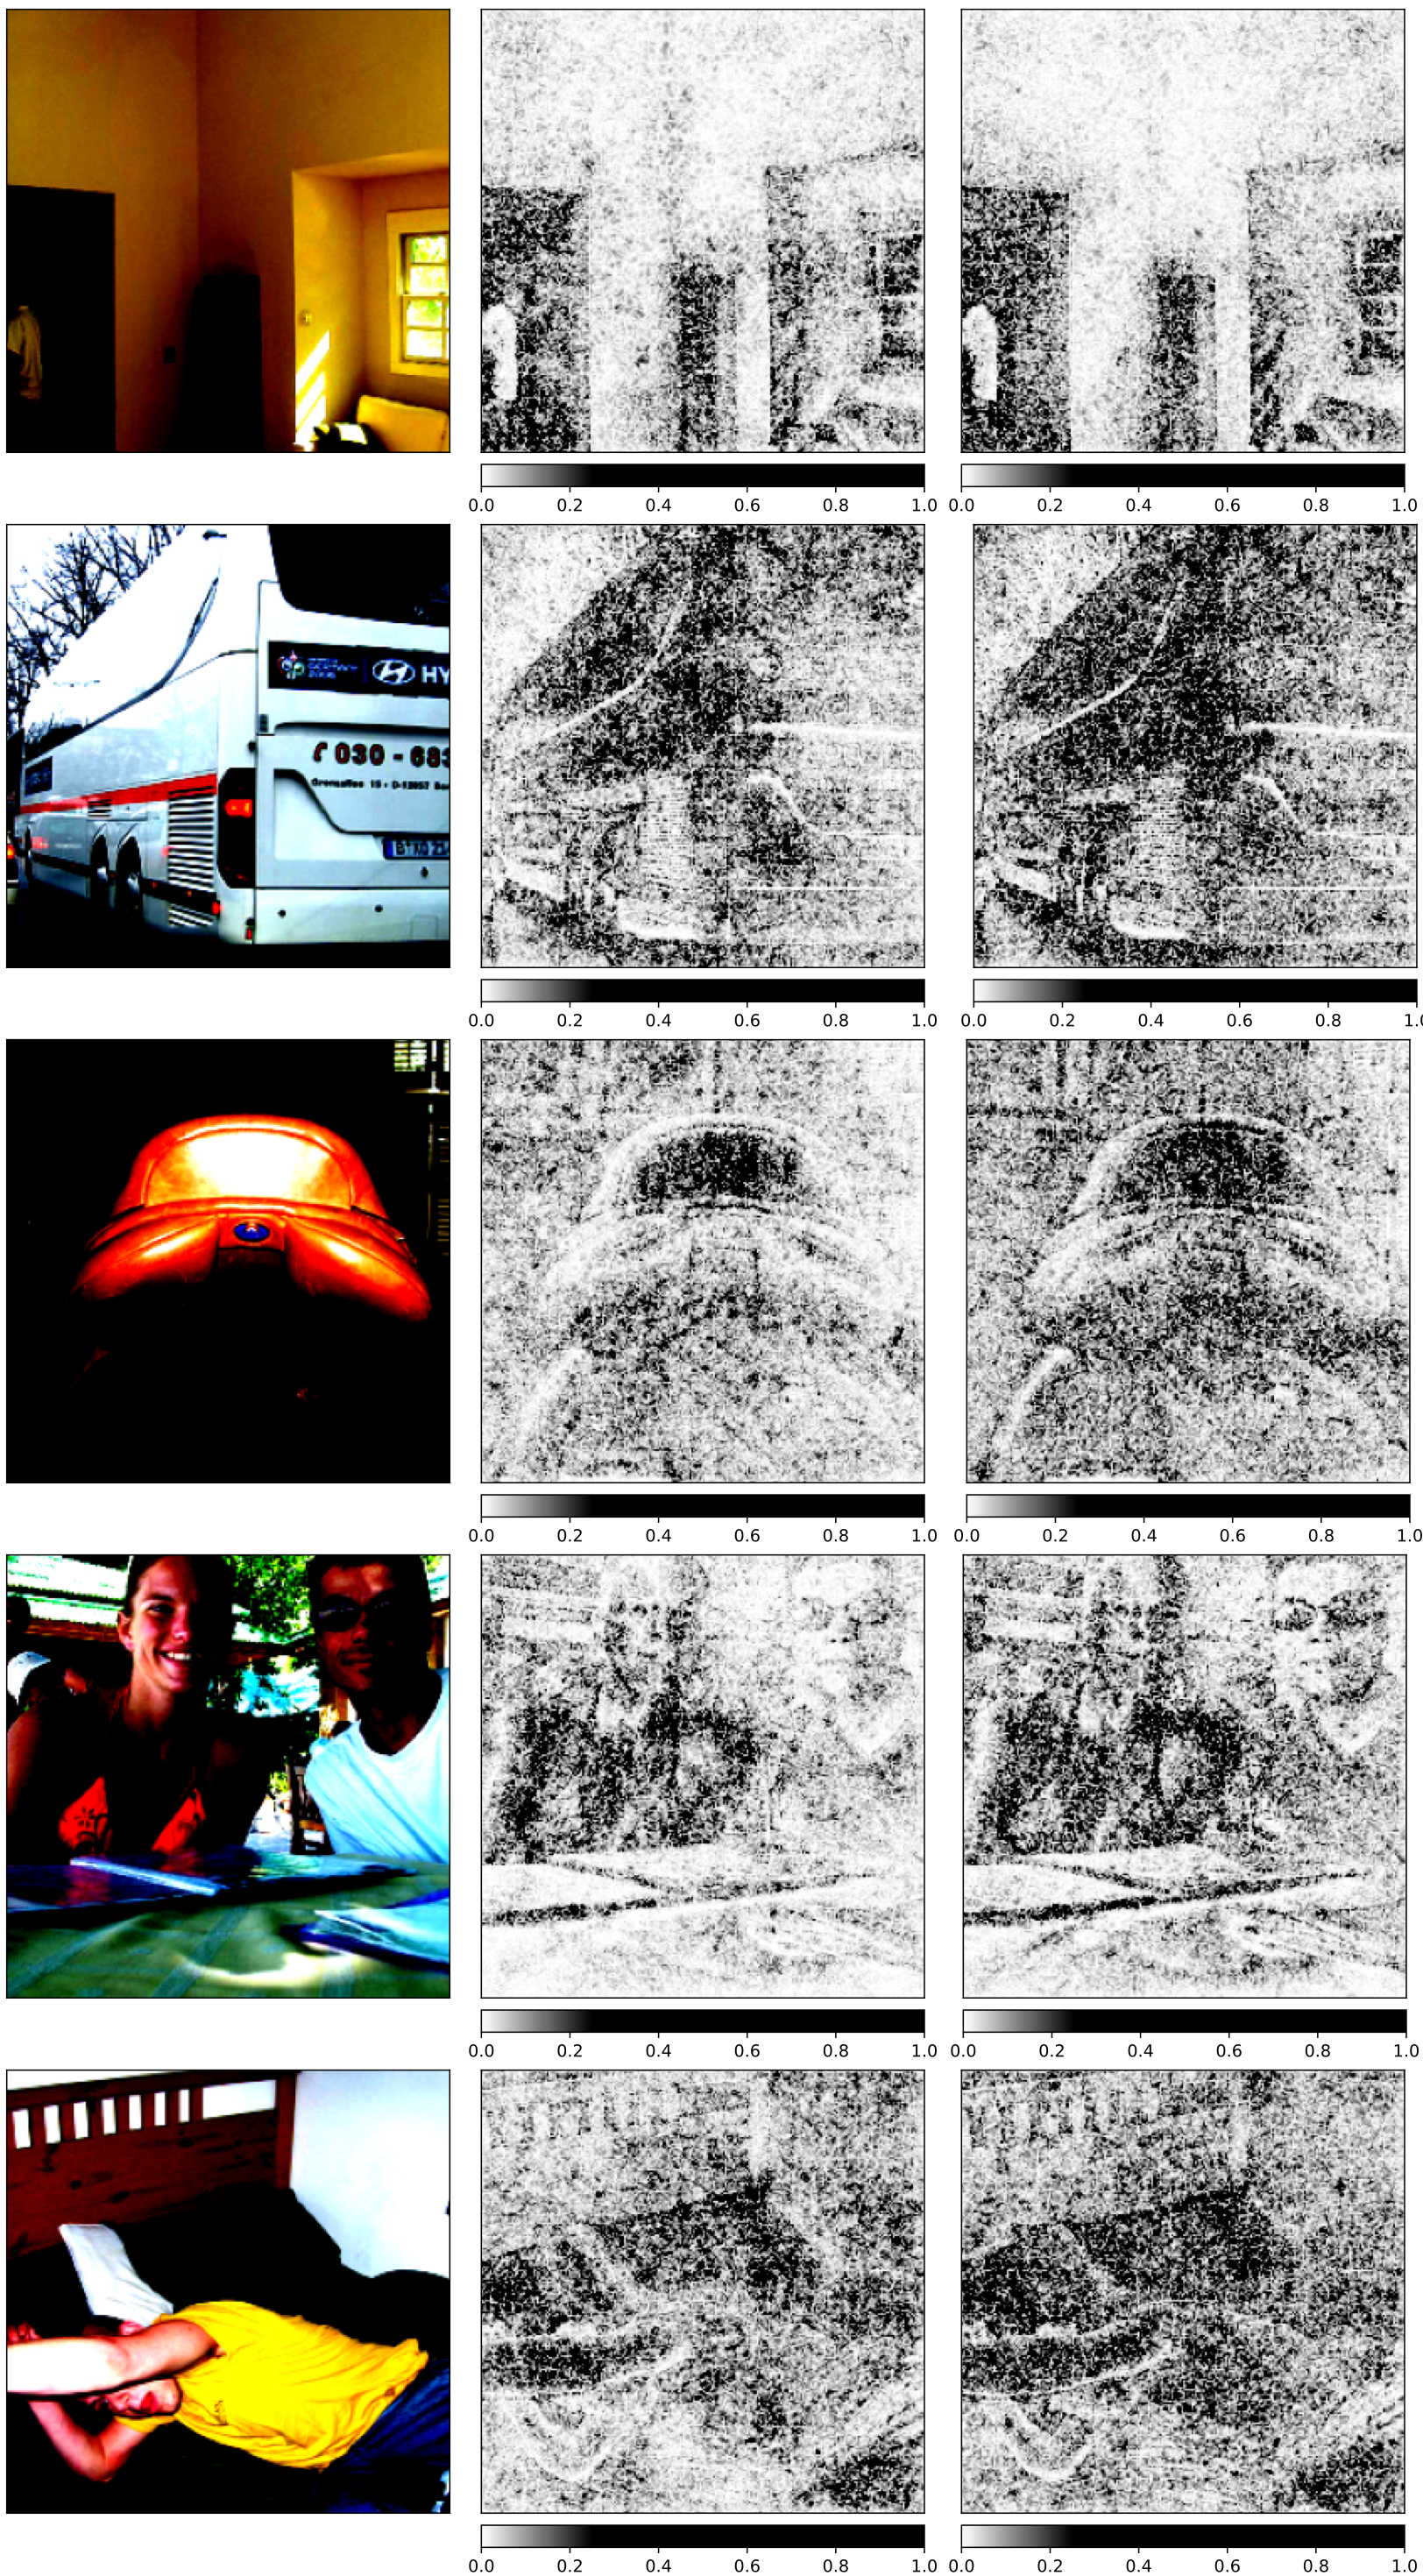
\includegraphics[width=0.52\textwidth]{figures/more_images.png}}
\caption{Heatmaps of Integrated Gradients (middle) and Geodesic IG (right) on 5 randomly chosen images from the test set of Pascal VOC 2012. We can see that Geodesic IG heatmaps are sharper compared with the original IG method.}
\label{fig:more_images}
\end{center}
\vskip -0.2in
\end{figure}
